\begin{figure}[htbp]
\centering
% Thesis-wide categorical color palette
% Usage: % Thesis-wide categorical color palette
% Usage: % Thesis-wide categorical color palette
% Usage: \input{figures/palette} in any figure file
%
% Muted primary colors -- print-friendly, visually distinct.
% Inspired by Cooper Union's red/blue primaries, softened for
% academic figures. Use palA-palC for data series in scatter
% plots, line charts, bar charts, etc.

\definecolor{palA}{HTML}{1F77B4}   % Tableau blue
\definecolor{palB}{HTML}{D62728}   % Tableau red
\definecolor{palC}{HTML}{2CA02C}   % Tableau green
 in any figure file
%
% Muted primary colors -- print-friendly, visually distinct.
% Inspired by Cooper Union's red/blue primaries, softened for
% academic figures. Use palA-palC for data series in scatter
% plots, line charts, bar charts, etc.

\definecolor{palA}{HTML}{1F77B4}   % Tableau blue
\definecolor{palB}{HTML}{D62728}   % Tableau red
\definecolor{palC}{HTML}{2CA02C}   % Tableau green
 in any figure file
%
% Muted primary colors -- print-friendly, visually distinct.
% Inspired by Cooper Union's red/blue primaries, softened for
% academic figures. Use palA-palC for data series in scatter
% plots, line charts, bar charts, etc.

\definecolor{palA}{HTML}{1F77B4}   % Tableau blue
\definecolor{palB}{HTML}{D62728}   % Tableau red
\definecolor{palC}{HTML}{2CA02C}   % Tableau green


\begin{subfigure}[t]{0.45\textwidth}
\centering
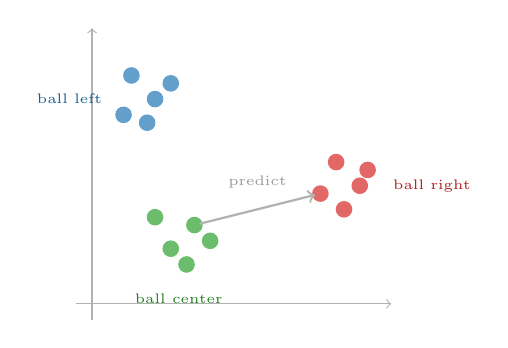
\begin{tikzpicture}[
    lbl/.style={font=\scriptsize, text=black!55},
]

% Axes
\draw[->, black!30] (-0.2, 0) -- (3.8, 0);
\draw[->, black!30] (0, -0.2) -- (0, 3.5);

% Cluster 1: "ball left" states (palA blue) -- upper left
\fill[palA!70] (0.5, 2.9) circle (3pt);
\fill[palA!70] (0.8, 2.6) circle (3pt);
\fill[palA!70] (0.4, 2.4) circle (3pt);
\fill[palA!70] (1.0, 2.8) circle (3pt);
\fill[palA!70] (0.7, 2.3) circle (3pt);

% Cluster 2: "ball center" states (palC green) -- lower left
\fill[palC!70] (1.0, 0.7) circle (3pt);
\fill[palC!70] (1.3, 1.0) circle (3pt);
\fill[palC!70] (0.8, 1.1) circle (3pt);
\fill[palC!70] (1.2, 0.5) circle (3pt);
\fill[palC!70] (1.5, 0.8) circle (3pt);

% Cluster 3: "ball right" states (palB red) -- right
\fill[palB!70] (3.1, 1.8) circle (3pt);
\fill[palB!70] (3.4, 1.5) circle (3pt);
\fill[palB!70] (2.9, 1.4) circle (3pt);
\fill[palB!70] (3.5, 1.7) circle (3pt);
\fill[palB!70] (3.2, 1.2) circle (3pt);

% Cluster labels -- positioned away from dots
\node[font=\tiny, text=palA!80!black, anchor=east]
    at (0.25, 2.6) {ball left};
\node[font=\tiny, text=palC!80!black, anchor=north]
    at (1.1, 0.25) {ball center};
\node[font=\tiny, text=palB!80!black, anchor=west]
    at (3.7, 1.5) {ball right};

% Prediction arrow example (meaningful)
\draw[->, thick, black!30, shorten >=2pt, shorten <=2pt]
    (1.3, 1.0) -- (2.9, 1.4);
\node[font=\tiny, text=black!40, anchor=south]
    at (2.1, 1.35) {predict};

\end{tikzpicture}
\subcaption{Useful representations}
\label{fig:collapse-useful}
\end{subfigure}
\hfill
\begin{subfigure}[t]{0.45\textwidth}
\centering
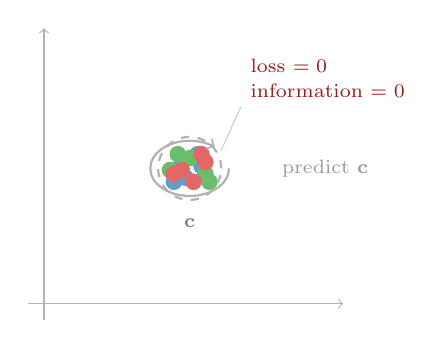
\begin{tikzpicture}[
    lbl/.style={font=\scriptsize, text=black!55},
]

% Axes
\draw[->, black!30] (-0.2, 0) -- (3.8, 0);
\draw[->, black!30] (0, -0.2) -- (0, 3.5);

% All points collapsed to center -- spread enough to see colors
\fill[palA!70] (1.75, 1.80) circle (3pt);
\fill[palA!70] (1.95, 1.90) circle (3pt);
\fill[palA!70] (1.65, 1.55) circle (3pt);
\fill[palA!70] (2.00, 1.75) circle (3pt);
\fill[palA!70] (1.80, 1.60) circle (3pt);

\fill[palC!70] (2.05, 1.65) circle (3pt);
\fill[palC!70] (1.85, 1.85) circle (3pt);
\fill[palC!70] (1.60, 1.70) circle (3pt);
\fill[palC!70] (2.10, 1.55) circle (3pt);
\fill[palC!70] (1.70, 1.90) circle (3pt);

\fill[palB!70] (2.05, 1.80) circle (3pt);
\fill[palB!70] (1.75, 1.70) circle (3pt);
\fill[palB!70] (1.90, 1.55) circle (3pt);
\fill[palB!70] (2.00, 1.90) circle (3pt);
\fill[palB!70] (1.65, 1.65) circle (3pt);

% Highlight the collapse cluster
\draw[black!30, thick, dashed]
    (1.85, 1.72) circle (0.40);

% Constant vector label
\node[font=\scriptsize, text=black!50, anchor=north]
    at (1.85, 1.2) {$\mathbf{c}$};

% Annotation: loss = 0, information = 0
\node[font=\scriptsize, text=palB!70!black, align=left,
    anchor=south west] at (2.5, 2.5)
    {loss $= 0$\\[1pt] information $= 0$};
\draw[thin, black!20] (2.25, 1.95) -- (2.5, 2.5);

% Trivial prediction (self-loop, larger)
\draw[->, thick, black!30]
    (2.35, 1.72) arc[start angle=0, end angle=-310,
    x radius=0.5, y radius=0.35];
\node[font=\scriptsize, text=black!40, anchor=west]
    at (2.9, 1.72) {predict $\mathbf{c}$};

\end{tikzpicture}
\subcaption{Collapsed representations}
\label{fig:collapse-collapsed}
\end{subfigure}

\caption{Representational collapse. (a)~The encoder maps different
  game states to distinct regions, preserving meaningful structure.
  (b)~Under collapse, all states map to the same constant
  vector~$\mathbf{c}$: prediction is trivially correct but the
  representation carries no information.}
\label{fig:collapse}
\end{figure}
